\chapter{Điều khiển và sao chép dữ liệu với Raspberry Pi}
%Có một cách có thể dùng để điều khiển Raspberry Pi
\section{Điều khiển bằng cách kết nối trực tiếp với màn hình, bàn phím và chuột}
\begin{itemize}
\item \textit{Điều khiển}: Kết nối chuột và bàn phím qua các cổng USB. Với màn hình thông thường có 2 loại: màn hình hỗ trợ cổng HDMI và màn hình hổ trợ cổng VGA.
\item \textit{Sao chép dữ liệu}: Sử dụng USB.
\end{itemize}
\subsection{Màn hình hổ trợ cổng HDMI}
Ta kết nối màn hình qua cable HDMI. Có thể bạn sẽ cần tùy chỉnh một số thông sau cho phù hợp:
\subsection{Màn hình hổ trợ cổng VGA}
Để hiển thị được, ta cần có cable chuyển đồi từ VGA sang HDMI.
\begin{figure}[!h]
\begin{center}
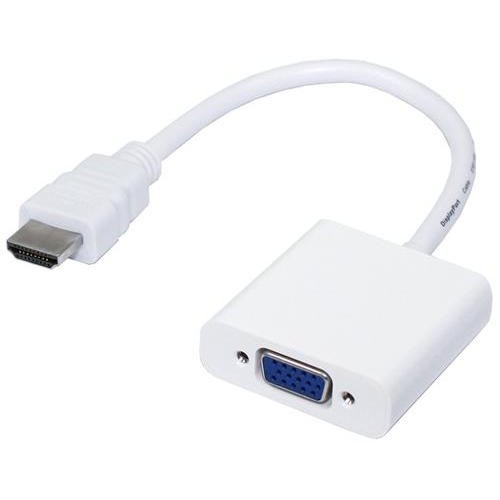
\includegraphics[scale=.3]{remote/images/HDMI-VGA-white}
\end{center}
\caption{Cáp chuyển đổi từ cổng HDMI sang cổng VGA}
\end{figure}
\section{Điều khiển bằng giao tiếp nối tiếp thông qua cổng RS232} \label{Sec:rs232}
Khi kết nối bằng module RS232, cần cấp nguồn cho Pi hoạt động.
\begin{figure}[!h]
\begin{center}
\subfloat[Module RS232 to TTL]
  {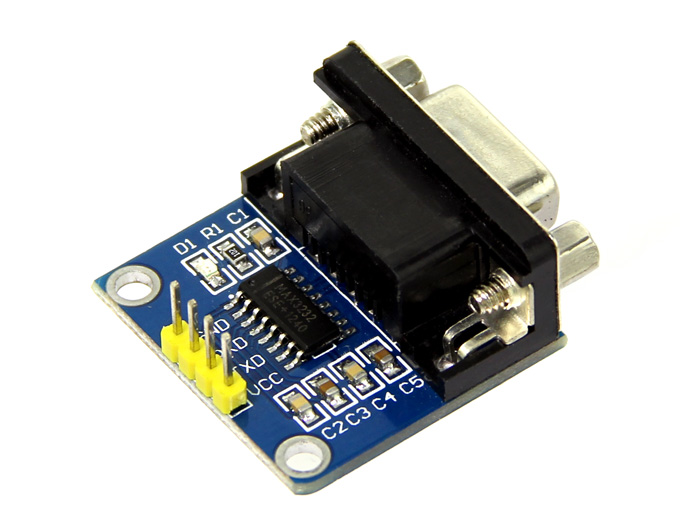
\includegraphics[width=.3\linewidth]{remote/images/RS232-to-ttl}}\hspace{1cm}
\subfloat[Cáp USB to COM]
  {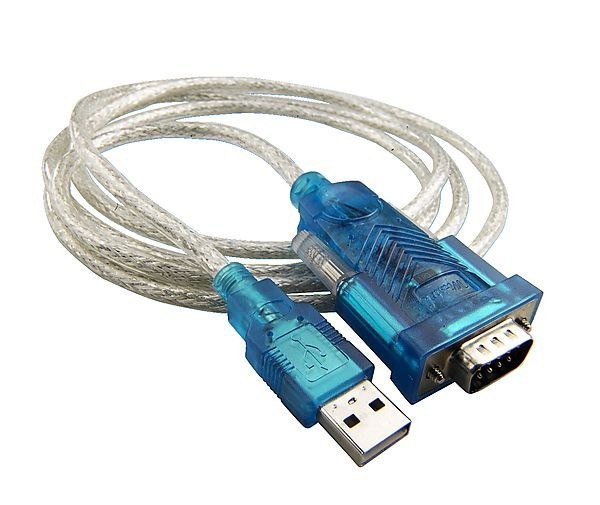
\includegraphics[width=.3\linewidth]{remote/images/cap-usb-to-com}}
\end{center}
\caption{Module RS232 to TTL và Cáp USB to COM}
\end{figure}
\begin{itemize}
\item Thực hiện kết nối Pi và module RS232 như sau:
\begin{center}
\begin{tabular}{c|c}
Pi & RS232\\ \hline
3.3V & VCC\\
TX & TX \\ 
RX & RX\\
GND & GND
\end{tabular}
\end{center}
\item Cài đặt gói phần mềm \verb|screen|: \verb|sudo apt-get install screen| trên máy tính Ubuntu.
\item Chạy lệnh sau: \verb|sudo screen /dev/ttyUSB0 115200|
\item Thực hiện xong lệnh trên, ta nhấn Enter một lần nữa để kết nối với Pi.
\item Nhập username và password để đăng nhập.
\item Sao chép dữ liệu: dùng USB.
\item[$\ast$] Ta có thể dùng Putty (trên hệ điều hành Window) để điều khiển: chọn \verb|Serial|, điền vào khung \verb|Serial line| tên cổng (ví dụ: COM1, COM2,\ldots), trong khung \verb|Speed| điền tốc độ là \verb|115200|. Nhập username và password để đăng nhập.
\end{itemize}
\section{Điều khiển bằng giao tiếp nối tiếp thông qua cáp USB to COM PL2303}
Khi kết nối bằng cáp USB to COM PL2303 thì không cần cấp nguồn ngoài cho Pi hoạt động (do Pi sẽ lấy nguồn từ cổng USB thông qua cáp).
\begin{figure}[!h]
\begin{center}
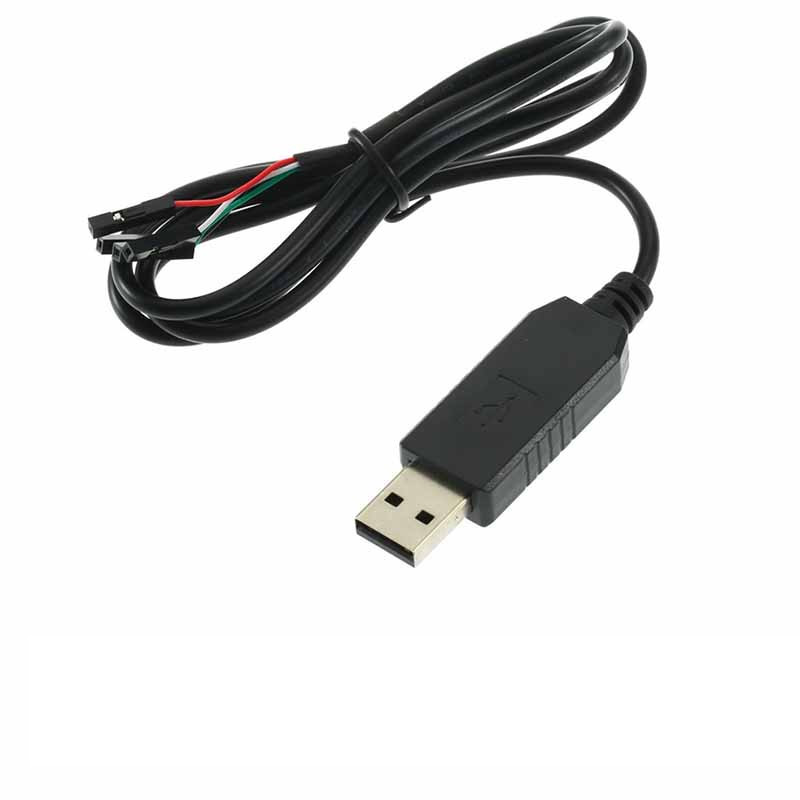
\includegraphics[scale=.3]{remote/images/cap-usb-to-com-pl2303}
\end{center}
\caption{Cáp USB to COM PL2303}
\end{figure}
\begin{itemize}
\item Thực hiện kết nối Pi và cáp USB to COM PL2303 như sau:
\begin{center}
\begin{tabular}{c|c|c}
Pi & PL2303 & Màu dây\\ \hline
5V & VCC & Đỏ\\
TX & RX & Trắng\\ 
RX & TX & Xanh\\
GND & GND & Đen
\end{tabular}
\end{center}
\item Phần cài đặt và điều khiển tương tự như cổng RS232 (xem \textit{mục \ref{Sec:rs232} trang \pageref{Sec:rs232}}).
\end{itemize}
\section{Điều khiển từ xa khi Raspberry Pi có kết nối mạng}
Khi Raspberry Pi có kết nối mạng Internet, ta có thể dùng các phần mềm: \verb|SSH|, \verb|Remote Desktop|, \verb|VNC|,\ldots~ để điều khiển.
\begin{itemize}
\item Kiểm tra địa chỉ IP của Pi bằng phần mềm: ipscan (trên Windows) hoặc nmap (trên Ubuntu).
\item Chọn chương trình phù hợp để điều khiển Raspberry Pi: 
\begin{itemize}
\item Với \verb|SSH|: không hổ trợ giao diện đồ họa.
\item Với \verb|Remote Desktop| (Pi cần cài đặt: \verb|xrdp|, dùng lệnh: \verb|sudo apt-get install xrdp|), \verb|VNC|: có hổ trợ giao diện đồ họa.
\end{itemize}
\item Tùy theo chương trình bạn chọn: ta cần phải nhập địa chỉ IP, username và password (nếu có yêu cầu điền số \verb|port|: ta điền 22).
\item Sao chép dữ liệu:
\begin{itemize}
\item Trên Window: dùng \verb|Winscp|.
\item Trên Ubuntu: dùng \verb|FileZilla|.
\item[$\ast$] Ta cũng cần nhập vào thông tin như trên để truy cập được Pi.
\end{itemize}
\item \textit{Lưu ý}: Phần trình bày trên áp ngay cho mạng nội bộ, khi không phải mạng nội bộ ta cần cấu hình mạng rồi mới áp dụng được hướng dẫn ở phần này.
\end{itemize}

